\chapter{Directional Noise Elimination}\label{ch:directional}
\section{Introduction}
This chapter deals with directional filtering. The idea is presented and tested. The 
results and conclusions will be shown afterwards.
\section{Concept}
Figure \ref{fig:2sources} shows a scenario where directional filtering could be used.
Source 1 and Source 2 are both talking simultaneously. At the Origin, two microphones 
left(L) and right(R) are recording both signals.

\begin{figure}[htp]
	\centering
	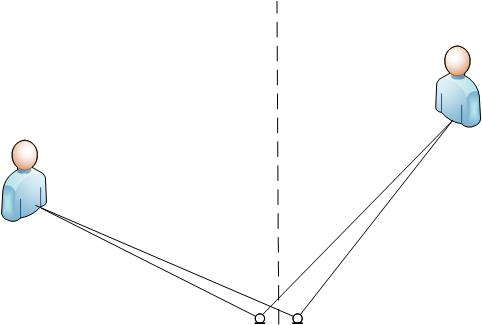
\includegraphics[width=0.65\textwidth]{Illustrations/2sources.jpg}
	\caption{Two Persons Talking}
	\label{fig:2sources}
\end{figure}

Due to the placement of the sources, both microphones will record the sounds, with a 
certain delay.

\section{Idea for filtering}

\begin{figure}[htp]
	\centering
	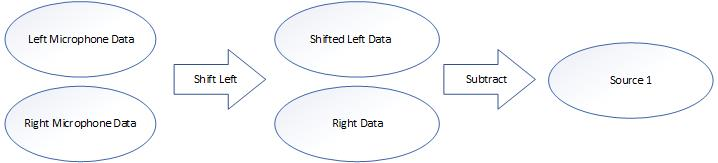
\includegraphics[width=1\textwidth]{Illustrations/IdeaDiagram.jpg}
	\caption{Idea diagram}
	\label{fig:IdeaDiagram}
\end{figure}

Filtering sound, based on the direction that it's coming from could work by taking data, recorded by one of the microphones, in this case (figure
\ref{fig:IdeaDiagram}) we chose left microphone data. Then we shift this data by exact amount of samples, which would make the source we would like 
to separate recorded by left microphone, exactly aligned with same source, recorded by right microphone.\\
Then by subtracting right microphone data from shifted left, we should get all the other sounds except the ones from source we would like to
separate, this is what we will call noise in directional filtering.\\
Separating could be done by taking the original data, putting it to one channel. Then subtracting noise from the original data should leave us only
with "clean" sound from the direction, we are interested in.\\
\section{Development}
\todo{MENTION WHERE EACH SUBSECTION COMES IN PLAY}
\subsection{Finding delay in samples}
By setting the angle of what we want to separate our signal at, we can calculate how big shift in samples that would account for. We are using this 
delay later, in the directional filtering. Calculations involve using selected angle, gap between microphones, sampling frequency of used 
microphones and the 
speed of sound. \\
\todo{DO WE WRITE ABOUT MATH AND EQUATIONS IN MATLAB HERE OR DO WE JUST SKIP IT.}

\subsection{Filtering}
All of the directional filtering is done by applying the logic in the figure
\section{Conclusion}